\documentclass{article}
\usepackage[utf8]{inputenc}
\usepackage[T1]{fontenc}
\usepackage[french]{babel}
\usepackage{graphicx}
\usepackage{soul}
\usepackage{color}
\newcommand{\hilight}[1]{\colorbox{red}{#1}}

\title{visualisation}
\author{yves.noblet }
\date{January 2023}

\begin{document}

\maketitle

\section{L’impact des guerres du xx\up{e} siècle sur les populations}
Les graphiques ci-dessous vont permettre d'apporter des éléments de réponse à la question suivante : quel a été l'impact des guerres du xx\up{e} siècle sur les populations ? 
Pour répondre à cette question, nous faisons face à certaines difficultés, notamment d'un point de vue technique, ou matériel. En effet, si la Belgique a participé aux deux guerres mondiales, les données concernant le nombre de décès manquent pour les années 1914 à 1918, ce qui fait que la partie des courbes chronologiques portant sur ces données, et correspondant à cette période, ne nous apprendront rien. 
L'impact des guerres n'a pas été le même pour les trois pays. Comme dit précédemment, la Belgique a pris part aux deux conflits mondiaux, notamment d'un point de vue militaire avec la mobilisation de son armée et sa participation aux combats. Il n'en va pas tout à fait de même pour la Finlande et la Norvège. Cette dernière s'est en effet déclarée neutre durant la première guerre mondiale\cite[p. 45]{knutsen1999norway}. Toutefois, elle a plutôt tenu une position en faveur de la Triple Entente. En effet, son économie était davantage tournée vers le Royaume-Uni, or la Norvège avait déjà fait les frais d'un blocus effectué par la marine britannique durant les guerres napoléoniennes, ce qui l'a donc poussé à plutôt mener une politique de bon entente avec le Royaume-Uni \cite[p. 46]{knutsen1999norway}. La guerre n'a cependant pas épargné l'économie norvégienne, qui s'est retrouvée face à des problèmes aux niveaux économique et alimentaire, avec, de plus, un accroissement des inégalités sociales\cite[pp. 48-49]{knutsen1999norway}. La Norvège s'est cependant retrouvée impliquée dans la seconde guerre mondiale en étant envahie par l'armée allemande en 1940 et occupée jusqu'en 1945. La Finlande, quant à elle, faisait partie de l'empire russe jusqu'à la déclaration de son indépendance peu de temps après le déclenchement de la révolution russe en 1917\cite{Maavara2016Revolution}. Bien que faisant partie de l'empire russe, qui s'est retrouvé militairement impliqué dans la première guerre mondiale, très peu de Finlandais ont participé aux combats. Les Finlandais n'étaient pas concernés par la conscription russe, ainsi seuls 800 Finlandais se sont engagés volontairement dans l'armée impériale russe. Par ailleurs, en raison d'un mouvement anti-russe, environ 2000 Finlandais se sont rendus en Allemagne afin de s'engager dans l'armée allemande et combattre l'armée russe. D'un point de vue militaire, la Finlande s'est donc retrouvée peu impactée par la première guerre mondiale\cite{Maavara2016FirstWorldWar}. Cependant, suite à la révolution russe, après la déclaration de son indépendance en décembre 1917, la Finlande traverse elle aussi une période de guerre civile au cours de l'année 1918 qui, comme nous allons le voir, a eu un certain impact sur la population\cite{Maavara2016CivilWar}. Par la suite, la Finlande s'est retrouvée fortement impliquée dans la seconde guerre mondiale. Durant l'hiver 1939-1940, elle entre en conflit armé avec l'Union soviétique, un conflit qui restera connu comme sous le nom de "guerre d'Hiver". Après une trêve d'un an avec l'Union soviétique, la Finlande reprend les armes contre l'Union soviétique aux côtés de l'Allemagne lorsque cette dernière envahit l'Union soviétique en juin 1941, cette "guerre de Continuation", durera jusqu'en septembre 1944, lorsqu'un armistice est signé à Moscou. Suite à cet armistice avec Moscou, les combats ne cessent pas et les Finlandais doivent désormais chasser les forces allemandes présentes sur leur territoire, principalement en Laponie finlandaise, selon les termes de l'armistice signé à Moscou\cite[pp. 5-17]{jowett2012finland}. 
\subsection{L'impact sur les décès}
\subsubsection{Décès totaux}
\begin{figure}[htbp]
\centering
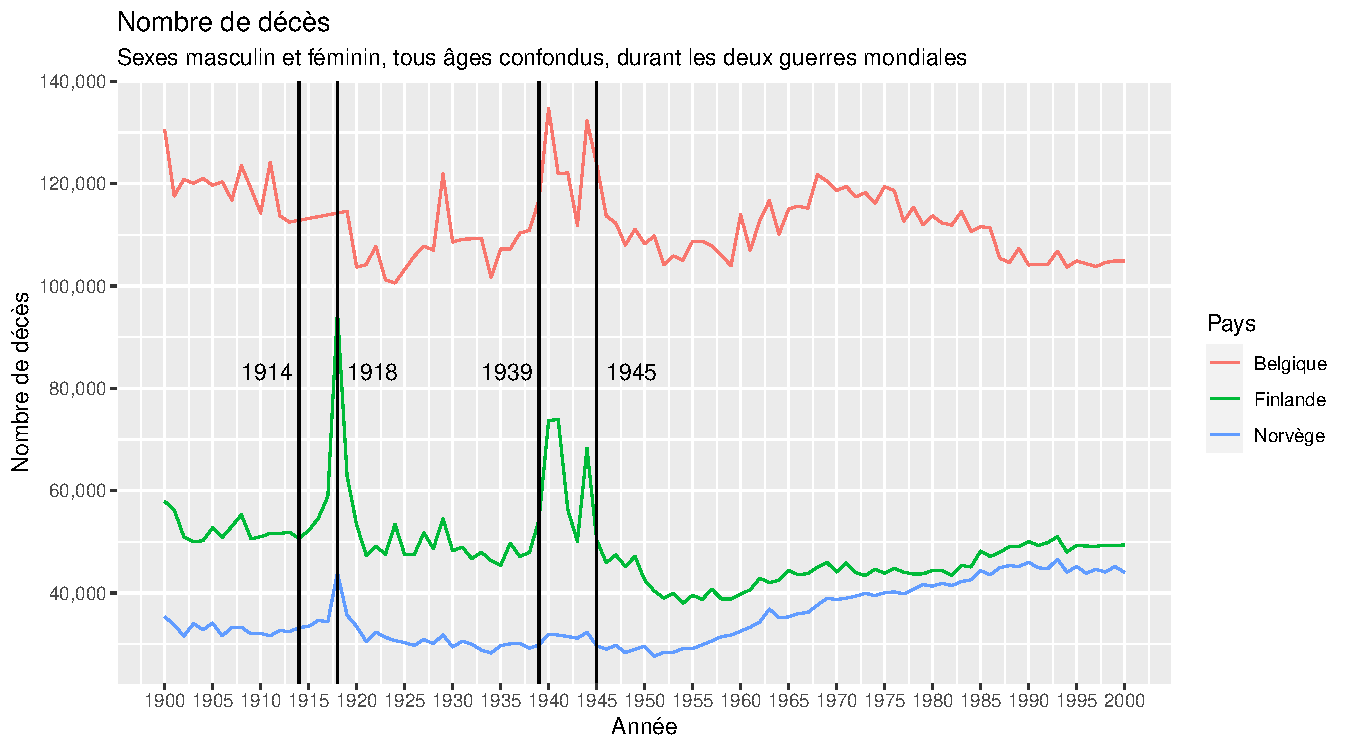
\includegraphics[width=\linewidth]{graph_nbrmorts_total.pdf}
\end{figure}
\paragraph{}
Commentaire sur la conception du graphique : 
\paragraph{}
Pour ce premier graphique, j'ai décidé de m'intéresser au nombre de décès durant les deux guerres mondiales et la guerre civile finlandaise. Pour ce faire, j'ai créé un sous-data dans lequel j'ai sélectionner la modalités "Deaths" pour la colonne "Variable", les années 1900 à 2000 pour la colonne "Year" et la modalité "Total" pour la colonne "Sex". Le but de graphique est de voir l'impact des guerres sur le nombre de décès, autant pour le sexe masculin que féminin, pour tous les âges confondus. Pour la conception de ce graphique, j'ai choisi de prendre une courbe chronologique, tout comme c'est le cas pour les autres graphiques portant sur cette question de l'impact des guerres du xx\up{e} siècle sur les populations. Pour répondre à cette question, il m'a en effet paru être plus judicieux de voir les impacts en comparaison avec le reste du xx\up{e} siècle. Or la courbe chronologique permet de confronter les données disponibles pour les deux guerres mondiales à celles du reste du xx\up{e} siècle. Elle permet donc de prendre pleinement conscience de l'étendue des impacts qu'ont eu ces guerres sur les populations. Comme correspondances visuelles, j'ai indiqué comme aes((x=Year, y= Value, color= Country). Cependant, un problème se présentait dans le graphique dû à l'agencement du tableau de données disponible. En effet, dans le tableau de données, une colonne contenant la variable "Age" reprenait tous les âges de 0 à 109. ce qui fait que pour chaque année il y avait 110 lignes de données, que le logiciel essayait de relier toutes en même temps ce qui donnait un résultat très peu satisfaisant. Pour remédier à cela, il a suffi d'agréger les âges, en partant de notre premier sous-data, ce qui a permis d'avoir un autre sous-data pour lesquels nous avions une colonne pour l'année, une pour le pays et une pour les valeurs. Pour les couleurs des courbes, dans un soucis d'uniformisation, \hilight{nous avons décidé de laisser les couleurs par défaut}. Concernant les échelles, pour l'axe des x, à l'aide de l'option limits, j'ai fixé les limites de l'axe des x de 1900 à 2000. Pour la graduation, étant donné que les guerres qui nous intéressent se sont déroulées sur des périodes de 4 à 6 ans, il m'a semblé pertinent de placer les graduations par intervalle de 5 ans afin de faciliter la lecture pour les périodes qui nous intéresse. Pour l'axe des y, j'ai laissé les limits et breaks par défaut et pour les labels, j'ai précisé comma dans l'instruction scale\_y\_continuous. Le paramtère par défaut aurait autrement indiqué les chiffres de la manière suivante : 100000, ou encore 1e+6 pour un 1.000.000. Ainsi, afin de faciliter la lecture, j'ai préféré utiliser la fonction comma pour l'option labels. Enfin, afin de faire ressortir les périodes de guerre et de mettre l'accent sur ces données,des droites de références, indiquant précisément les années 1914, 1918, 1939 et 1945 ont été placées. 
\paragraph{}
Bref commentaire du phénomène observé : 
Pour des raisons évoquées précédemment, la partie de la courbe concernant la Belgique pour les années 1914 à 1918 n'est pas à prendre en compte étant donné l'absence des données dans le data. Cependant, on peut clairement voir pour le reste que les conflits ont eu un net impact sur la mortalité. Pour la Belgique, il est nettement visible que le nombre de décès a été plus élevé durant la seconde guerre mondiale que durant le reste du xx\up{e} siècle. En particulier pour les années 1940 et 1944, ce qui est normal étant donné qu'il s'agit des années au cours desquelles des combats ont eu lieu en Belgique. Ainsi, durant le mois de mai 1940, l'armée allemande a envahi la Belgique et c'est en 1944 qu'elle est chassée par l'arrivée des troupes alliées. Pour la Finlande, on peut voir nettement l'impact de la guerre civile de 1918 sur le nombre des décès, de même que celui de la guerre d'Hiver de 1939-1940 et par la suite de la guerre de continuation qui dure jusqu'en 1944, on peut d'ailleurs nettement voir sur le graphique que le nombre de décès diminuent entre 1944 et 1945. Concernant la Norvège, étant donné qu'elle n'a pas participé la première guerre mondiale, on ne remarque pas de forte augmentation des décès, excepté pour les années 1917-1918, ce qui pourrait être dû à des pénuries alimentaires ou à des difficultés économiques rencontrées en raison du contexte géopolitique de l'époque. 
\subsubsection{Décès parmi les femmes}
\paragraph{}

\bibliographystyle{plain}
\bibliography{bibliographieVisualisation}
\end{document}
